\title{Midterm 1 for Calculus-Based Physics: Electricity and Magnetism}
\author{Dr. Jordan Hanson - Whittier College Dept. of Physics and Astronomy}
\date{\today}
\documentclass[10pt]{article}
\usepackage[a4paper, total={18cm, 27cm}]{geometry}
\usepackage{outlines}
\usepackage[sfdefault]{FiraSans}
\usepackage{hyperref}
\usepackage{graphicx}
\begin{document}
\maketitle

\textbf{Memory Bank:}
\begin{enumerate}
\item Coulomb Force: $\vec{F} = k \frac{q_1 q_2}{r^2}\hat{r}$
\item $k = 9 \times 10^{9}$ N C$^{-2}$ m$^{2}$
\item $q_e = 1.6 \times 10^{-19}$ C
\item Mass of a proton: $1.67 \times 10^{-27}$ kg
\item Electric field and charge: $\vec{F} = q \vec{E}$
\item Field of infinite wire of charge density $\lambda$: $\vec{E}(z) = \frac{2k\lambda}{z}\hat{z}$
\item Field of two oppositely charged infinite planes, with charge density $\sigma$: $\vec{E}(z) = \frac{\sigma}{\epsilon_0}\hat{z}$
\item $\epsilon_0 \approx 8.85 \times 10^{-12}$ F/m
\item Dipole moment: $\vec{p} = q \vec{d}$
\item Torque on dipole moment: $\vec{\tau} = \vec{p} \times \vec{E}$
\item Electric flux: $\Phi = \vec{E} \cdot \vec{A} = EA \cos\theta$
\item Gauss' law: $\Phi = Q_{enc}/\epsilon_0$
\item Potential energy and voltage: $U = q\Delta V$
\item Voltage of a point charge: $V(r) = k\frac{q}{r}$
\item Voltage and E-field: $\vec{E} = -\nabla V$, single-variable $\vec{E} = -\frac{dV}{dx}$
\item Constant E-field: $E = \frac{\Delta V}{\Delta x}$
\item E-field and voltage: $\Delta V = -\int \vec{E} \cdot d\vec{x}$
\item Capacitance: $Q = CV$
\item Parallel plate capacitor: $C = \frac{\epsilon_0 A}{d}$
\item Adding two capacitors in series: $C_{tot}^{-1} = C_1^{-1} + C_2^{-2}$
\item Adding two capacitors in parallel: $C_{tot} = C_1 + C_2$
\item Definition of current: $I(t) = \frac{dQ}{dt}$
\item Drift velocity: $v_d = \frac{I}{nAq}$
\item Ohm's law: $V = IR$
\item \textbf{Adding two resistors in series} $R_{tot} = R_1 + R_2$
\item \textbf{Adding two resistors in parallel} $R_{tot}^{-1} = R_1^{-1} + R_2^{-2}$
\end{enumerate}

\clearpage

\begin{enumerate}
\item \textbf{Chapter 5, Electrostatics}
\begin{enumerate}
\item Two electrons approach each other in space.  What is the electric force of repulsion between them when they are separated by $10^{-14}$ m? \\ \vspace{1cm}
\item A charge $q_1$ is located at (-2,0) in a 2D coordinate system, and a charge $q_2$ is located at (4,0).  If $2 q_1 = q_2$, find the value of the electric field at (0,0). \\ \vspace{2cm}
\item 
\begin{figure}
\centering
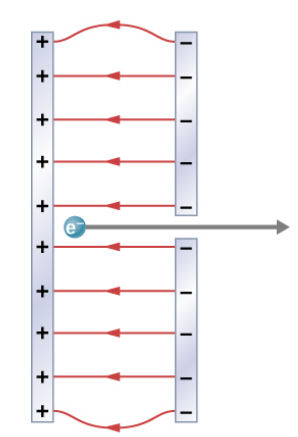
\includegraphics[width=0.2\textwidth]{figures/cap.png}
\caption{\label{fig:cap} A device accelerating a \textbf{positively charged} particle to the right.}
\end{figure}
In Fig. \ref{fig:cap}, assume a proton is being accelerated to the right.  (a) If the electric field is $E = 2000$ N/C to the right, what is the force on the proton?  (b) Using Newton's Second Law, show that the acceleration is $a = (q/m) E$.  (c)  Recall that an object that is accelerating travels a distance $d$ in a time $t$ according to $d = \frac{1}{2}at^2$.  How far has the proton travelled in 1 $\mu$s? \\ \vspace{3cm}
\end{enumerate}
\item \textbf{Chapter 6, Gauss' Law}
\begin{enumerate}
\item Derive (a) the electric field of a point charge using Gauss' Law.  (b) Derive the electric field versus $r$ of a solid sphere of constant charge density $\rho_0$ and radius $R$, for $r>R$.  (c) Do the results from (a) and (b) resemble each other? How? \\ \vspace{3cm}
\end{enumerate}
\item \textbf{Chapter 7, Voltage}
\begin{enumerate}
\item An arch of electricity sends 2.0 C of charge through a potential of $10^5$ Volts. What energy was dissipated? \\ \vspace{2cm}
\item Consult again Fig. \ref{fig:cap}.  (a) If the plates are 100 cm apart, and the field is still $2000$ N/C, what is the voltage difference between the plates? (b) Draw the voltage as a function of distance between the plates. \\ \vspace{2cm}
\end{enumerate}
\item \textbf{Chapter 8, Capacitance}
\begin{enumerate}
\item Find the charge stored when 5.0 V is applied to an 50.0 pF capacitor. \\ \vspace{1cm}
\item Find the charge stored when 5.0 V is applied to two 50.0 pF capacitors \textit{in parallel}. \\ \vspace{1cm}
\item Consult Fig. \ref{fig:cap2}.  If $C_1 = 50.0$ pF, $C_2 = 25.0$ pF, and $C_3 = 5.0$ pF, and $V=12.0$ Volts, what is the total charge? \\ \vspace{1.5cm}
\begin{figure}
\centering
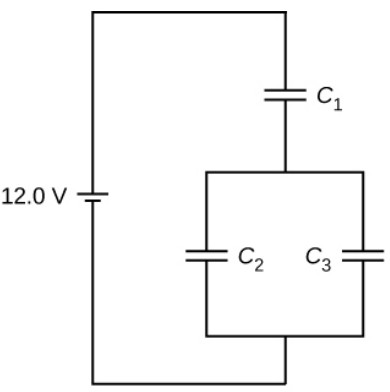
\includegraphics[width=0.2\textwidth]{figures/cap2.png}
\caption{\label{fig:cap2} A circuit of capacitors.}
\end{figure}
\end{enumerate}
\item \textbf{Chapter 9, Current and Ohm's law}
\begin{enumerate}
\item Suppose the charge collected in a capacitor is measured to follow the function $Q(t) = - Q_0 \exp(-t/\tau)$.  What is the current flowing into the capacitor? \\ \vspace{1cm}
\item Suppose two resistors $R_1=1$k$\Omega$ and $R_2=10$k$\Omega$ are connected \textit{in parallel} to a 5.0 V battery.  What is the current that flows from the battery?
\end{enumerate}
\end{enumerate}
\end{document}